\documentclass[conference]{IEEEtran}
%\IEEEoverridecommandlockouts

\usepackage{cite}
\usepackage{amsmath,amssymb,amsfonts}
\usepackage{algorithmic}
\usepackage{graphicx}
\usepackage{textcomp}
\usepackage{xcolor}
\usepackage{todonotes}
\usepackage{url}
\usepackage{microtype}
\usepackage{comment}
\usepackage[hidelinks]{hyperref}
\usepackage{flushend}

\usepackage{xspace}
\newcommand{\evosuite}{\textsc{EvoSuite}\@\xspace}
\newcommand{\tool}{\textsc{Tool}\@\xspace}
\usepackage{xcolor}
\usepackage{pifont}

\newcommand{\valerio}[1]{\textbf{\textcolor{blue}{[ \ding{46}Valerio: #1]}}}
\newcommand{\jens}[1]{\textbf{\textcolor{magenta}{[ \ding{46}Jens: #1]}}}
\newcommand{\tim}[1]{\textbf{\textcolor{violet}{[ \ding{46}Tim: #1]}}}
\newcommand{\behnaz}[1]
{\textbf{\textcolor{teal}{[ \ding{46}Behnaz: #1]}}}


\begin{document}

\title{Towards Cross-Build Regression Testing}

%\thanks{Identify applicable funding agency here. If none, delete this.}
% Valerio: this is for the camera ready version

\author{Anonymous Author(s)}
%Valerio: the track is double blind
\begin{comment}
\author{\IEEEauthorblockN{1\textsuperscript{st} Jens Dietrich  \hspace{1cm} 2\textsuperscript{nd} Tim White}
\IEEEauthorblockA{\textit{Victoria University of Wellington} \\
Wellington, New Zealand \\
\{jens.dietrich,tim.white\}@vuw.ac.nz}
\and
\IEEEauthorblockN{3\textsuperscript{rd} Valerio Terragni}
\IEEEauthorblockA{\textit{University of Auckland} \\
Auckland, New Zealand \\
v.terragni@auckland.ac.nz}
\and
\IEEEauthorblockN{4\textsuperscript{th} Behnaz Hassanshahi}
\IEEEauthorblockA{\textit{Oracle Labs Australia} \\
Brisbane, Australia \\
behnaz.hassanshahi@oracle.com}
}
\end{comment}

\maketitle

\begin{abstract}
\valerio{For the terminology we need to be a bit careful, if we are assuming that one of the jar we are comparing is correct, then is regression testing, otherwise if we are not making any assumption of what jar version is correct but we are just exposing behavioural differences than we are doing differential testing. Are we assuming that the jars in Maven Central are the correct ones ?  }
The purpose of generating regression tests is to detect behaviour changes as software evolves, therefore safeguarding against the introduction of bugs, and detecting changes that may break  clients downstream. We explore a different use case for regression testing – to detect behaviour changes  between different builds of the same version. This is motivated by concerns about software supply chain security that have led to the emergence of different binaries built from the same source code. We study this for TODO pairs of binaries built from the same source distributed using Maven Central, Google Assured Open Source Software and Oracle Build-From-Source. 
We find that ..

\end{abstract}

\begin{IEEEkeywords}
regression test generation, reproducible builds, software supply chain security
\end{IEEEkeywords}

\section{Introduction}

Software supply chain security has attracted increasing attention recently after a number of high impact attacks such as \textit{equifax}, \textit{log4shell}, \textit{solarwinds} and \textit{xz}~\cite{ellison2010evaluating,martinez2021software,enck2022top,EO14028}. In general, those fall into two categories - compromising components (such as \textit{equifax} and \textit{log4shell}), and compromising processes (such as \textit{solarwinds} and \textit{xz}). When build processes are compromised, attackers can inject malicious code into a program, resulting in a vulnerable program build from clean source code. The classic approach to achieve this is to compromise the compiler~\cite{thompson1984reflections}. 

A common counter measure are reproducible builds~\cite{reproduciblebuild, lamb2021reproducible}. The idea is to perform a second build leading to the same binary. As an adversary is very unlikely to compromise two build environments, this can confirm the integrity of the binary with a high probability. Establishing that the binaries are identical is usually done by means of bitwise comparison, often using cryptographic hashes as proxies.
Several organisations have started to provide infrastructure and services to provide such secondary builds at-scale, often meeting additional security-related requirements, such as SLSA compliance~\cite{slsa}. Two such products that include support for Java / Maven artifacts are \textit{Google's Assured Open Source Software (gaoss)}~\footnote{\url{https://cloud.google.com/security/products/assured-open-source-software}}, and \textit{Oracle's Build-From-Source (obfs})~\footnote{\url{https://maven.oracle.com/public/}}.

However, there are several challenges with the reproducibility of builds: (i) build environments are difficult to replicate, (ii) locating the source code version (commit, tag or release) associated with a binary release version is not always straightforward and (iii) builds may be non-deterministic~\cite{xiong2022towards,hassanshahi2023macaron,bineqdataset,keshani2024aroma}. In particular, different versions of compilers may employ different compilation strategies, resulting in different, yet functionally equivalent binaries~\cite{xiong2022towards,bineqdataset,schott2024JNorm}.  
In order to address this, recently bytecode normalisation techniques have been proposed~\cite{xiong2022towards,dietrich2024levelsbinaryequivalencecomparison,schott2024JNorm}. 

From a security analysis point of view, the comparison of binaries from alternative builds is used to detect vulnerabilities: different binaries may suggest that one of them has been compromised, for instance, by a backdoor being added during the build. A comparison based on strict binary equality is likely to result in poor precision as differences between binaries can be explained by the variability of compilers and other tools used in the build toolchain. Low precision is known to have a serious impact on the acceptance of program analysis tools by engineers~\cite{sadowski2018lessons,distefano2019scaling}. Using bytecode normalisation techniques such as \textit{jnorm}~\cite{schott2024JNorm} can help to reduce the false positive rate by identifying \textit{equivalent} binaries. The question arises whether binaries built from the same sources that are not equivalent actually have behavioural differences.   

This is the question we set out to study. We use test case generation with \evosuite~\cite{fraser2011evosuite} to synthesise regression tests for a baseline build, and then use those tests to assess whether these tests behave in the same way on programs that are the result of an alternative  build from the same sources. 

We find that .. 


\section{Methodology}



\subsection{Overview}

An overview of our methodology is depicted in Figure~\ref{fig:methodology}.  As a baseline build we use (the builds used to produce) the artifact distributed on Maven Central\footnote{\url{https://central.sonatype.com/}} as this is the default deployment repository for most open source developers.  From there we obtain the binary (jar file containing Java bytecode) \textit{mvnc jar} and the pom \textit{mvnc pom}. From this pom we extract the \textit{static dependencies} using the Maven dependency plugin~\footnote{\url{https://maven.apache.org/plugins/maven-dependency-plugin/}}.  The \textit{mvnc jar} and the \textit{static dependencies} can then be used as input to generate \textit{tests-sources} with \evosuite, which are then compiled into test binaries \textit{test-bin}.  Finally, those tests can then be executed against the original jar \textit{mvnc jar} and some alternative jar (from a different build) \textit{alt jar}, and the resulting test reports can be compared.

\begin{figure}[ht!]
	\centering
	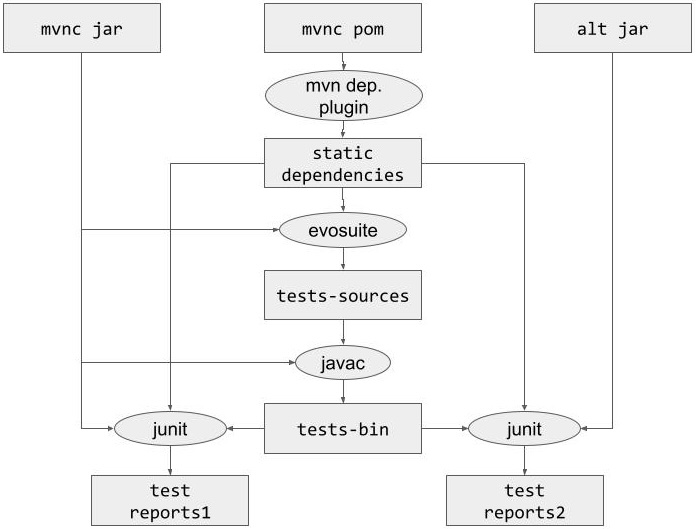
\includegraphics[width=\columnwidth]{methodology.jpg}
	\caption{Methodology Overview \label{fig:methodology}}
\end{figure}


\subsection{Project Selection}

We started with the dataset from \cite{dietrich2024levelsbinaryequivalencecomparison} that contains jars corresponding to the same artifact identified by the same group id, artifact id and version (i.e., GAV coordinates) built by different parties. This dataset contains the results of builds from Maven Central, Google (gaoss), Oracle (obfs) and  RedHat. We ignored jars built by RedHat as they have an additional patch id that suggests behavioural differences.  We only considered pairs where one of the jars was sourced from Maven Central, i.e. built by the developer(s). There are TODO such pairs.


\subsection{Static Preanalysis}

We then run a static pre-analysis to eliminate pairs that are probably equivalent. We first applied \textit{jnorm}, and compared jars by comparing the result of the transformation applied to each class. We then added a custom comparison based on a change in the Java 18 compiler~\footnote{\url{https://github.com/openjdk/jdk/pull/5165}} not yet supported by \textit{jnorm}. This resulted in TODO pairs of jars, TODO of those pairs with an alternatively built jar from \textit{gaoss}, TODO with such a jar from \textit{obfs}.



\subsection{Test Generation}

We opted to generate tests for these experiments. The reason is that existing tests that are part of the project are usually executed during builds, i.e., alternative builds would ensure that those tests succeed. 

\todo[inline]{Behnaz to confirm that tests are executed in OBF builds}

We used \evosuite to generate regression tests. While there are several alternatives available for Java, recent benchmarks have shown the superior performance of \evosuite~\cite{jahangirova2023sbft} in achieving higher code coverage and mutation scores. 

\valerio{I added some background on evosuite and regression testing in general, not sure where we want to put this but I think is important to explain how \evosuite exposes the behavioural differences}
\evosuite automatically generates test cases for a given object-oriented class under test (CUT). A test case consists of (i) a method call sequence that instantiates and modifies the state of objects of the CUT through method invocations (ii) one or more assertions that predicate on the values returned by the method invocations. The state of objects often dictates program behavior, so manipulating these states is crucial for achieving high coverage. It is worth noting that \evosuite may need to create and modify objects that do not instantiate the CUT, as the methods of the CUT might require non-primitive parameters. For primitive parameters, \evosuite uses randomized values guided by heuristics. The tool implements an evolutionary algorithm that evolves populations of test cases to maximize code coverage, typically targeting branch coverage.

\evosuite and similar automated testing tools are most effective when running in regression mode due to the oracle problem. In fact, they are predominantly evaluated in this mode~\cite{jahangirova2023sbft,shamshiri2015automatically}. While the oracle problem is one of the greatest challenges in test automation, it is mitigated in the context of regression testing, where we assume that one version is correct. In regression mode, \evosuite adds assertions to the generated test cases that capture the ``implemented'' behavior of the given version. These assertions are based on the actual values returned by method call invocations during execution, without regard for the ``intended'' behavior of the CUT. This approach can effectively expose behavioral differences between two implementations: if a test generated for one version fails on another version, it indicates a behavioral difference.

\evosuite can be set up to generate targeted tests for certain classes. Since the static pre-analysis compares \textit{jar} files by comparing the \textit{.class} files they contain, we can use targeted test generation for those classes only.   

\todo[inline] {Tim: some stats of how many classes there are that are different, perhaps stats , something like: the average number of such classes is X, Y\% of total classes. Mention how we deal with inner classes.  }

We run \evosuite test generation with the following settings. 

\todo[inline] {Tim: can you please provide details here, OS, JVM version, HW etc, plus evosuite settings in particular generation time}


Resource settings were informed by \cite{jahangirova2023sbft}. 



\section{Results}


\section{Related Work}

\emph{Differential Testing}\cite{difftesting} is an automated approach that identifies various errors by comparing the behavior of two or more comparable systems\cite{xie2007towards,jin10
,diffgen}. In the context of object-oriented (OO) programming, notable techniques include \textsc{Diffut}\cite{xie2007towards}, \textsc{BeRT}\cite{jin10
}, and \textsc{DiffGen}~\cite{diffgen}. Similar to our approach, these techniques leverage the differences between two software versions to generate test cases that reveal behavioral discrepancies. However, our approach focuses on comparing binaries, which required us to design and implement specialized ad-hoc analyses.

Although the implementation details may differ, all differential testing techniques share the core idea of generating and executing the same test cases on the versions being compared to reveal behavioral differences. % One of the most common applications of differential testing is regression testing, where two versions of the same program are compared. 
While differential testing has been effective in detecting semantic errors in various domains (e.g., C compilers~\cite{Yang:compiler:pldi:2011} and JVM implementations~\cite{Chen:jvmdiff:pldi:2016}), to the best of our knowledge, it has not yet been applied to identify differences between alternative builds of the same program version.






\section{Conclusion}








 \todo[inline]{complete}

\bibliographystyle{plain}
\bibliography{references}

\end{document}
